\documentclass[12pt]{article}
\usepackage[T1]{fontenc}
\usepackage{lmodern}
\usepackage[margin=1in]{geometry}
\usepackage{setspace,amsmath,amssymb,graphicx,booktabs,array,natbib,microtype}
\usepackage[font=small,labelfont=bf]{caption}
\usepackage[hidelinks,breaklinks]{hyperref}
\bibliographystyle{plainnat}
\setcitestyle{authoryear,round,aysep={}}
\onehalfspacing
\emergencystretch=3em
\setlength{\tabcolsep}{4pt}
\renewcommand{\arraystretch}{1.12}
\newcommand{\notes}[1]{\par\vspace{5pt}\begin{minipage}{.98\textwidth}\footnotesize\singlespacing #1\end{minipage}}
\newcommand{\HouseGap}{9.25}
\newcommand{\HouseCI}{[7.17, 11.35]}
\newcommand{\GeoChange}{0.39}
\newcommand{\GeoCI}{[-1.02, 1.60]}
\newcommand{\CondoGap}{0.77}
\newcommand{\CondoCI}{[-0.01, 1.56]}
\newcommand{\InitialGap}{11.42}
\newcommand{\PartyChange}{-2.32}

\title{\bfseries Who Gets the House?\\[2mm]\large Financing-Associated Price Gaps in New York City}
\author{}
\date{10 September 2026\\\small Working paper --- submission version WGTH-2026-09-10-JHE-S1}
\begin{document}
\maketitle
\begin{abstract}\singlespacing\noindent
How much of the observed price difference between cash and financed home purchases survives controls for changing transaction circumstances? New York City repeat sales show a house financing-associated gap of \HouseGap{} log points after permit restrictions, institutional-name exclusions, buyer and seller controls, and neighbourhood-time effects. The condominium contrast is much smaller under a common specification. Instrument checks expose limits to distress flags and co-operative financing assignments. The results document persistent conditional price differences, while leaving their division among execution risk, liquidity, changing condition and selection unidentified.
\end{abstract}
\noindent\textit{JEL:} H23, H71, R21, R31.\quad\textit{Keywords:} cash purchases; mortgage finance; repeat sales; housing prices; transaction selection.
\newpage

\section{Introduction}
Cash and financed buyers can pay different prices for the same home, but the difference need not measure the value of avoiding a failed mortgage-funded closing. Distress, improvements and buyer or seller selection can also change between sales. This paper asks how much of the financing-associated price gap remains after these observable transaction circumstances and local appreciation are considered together.

The central contribution is a cumulative repeat-sales assessment with jointly estimated uncertainty. New York City's financing-dependent mortgage recording tax supplies institutional motivation, but the observed financing switch is not an exogenous tax change. The analysis therefore estimates a conditional price contrast rather than a causal tax effect or an execution-risk premium.

The repeat-sales analysis uses an archived panel of 249,395 house and condominium sales in Manhattan, the Bronx, Brooklyn and Queens. It compares the price appreciation of properties switching from cash to financed purchase with those switching in the opposite direction. A cumulative specification sequence adds permit restrictions, institutional-name exclusions, buyer and seller type controls, and neighbourhood-by-time effects. The financing-switch indicators are fitted jointly with the market-price controls, and uncertainty in changes across specifications is estimated jointly on the same original parcel clusters.

The joint house contrast starts at \InitialGap{} log points and is \HouseGap{} after the full sequence, with a 999-refit parcel-bootstrap interval of \HouseCI{}. Buyer and seller type controls reduce the contrast. Neighbourhood appreciation does not explain it away: on identical linked pairs, adding ZIP-year effects changes the joint coefficient by \GeoChange{} log points, with interval \GeoCI{}. The original procedure, which removes market controls only from the outcome before comparing switching-group means, yields a different statistic. Its decline after adding geographic controls is not the contribution of local appreciation to the jointly estimated coefficient.

The condominium contrast under the common borough-quarter specification is much smaller, at \CondoGap{} log points with interval \CondoCI{}. Co-operative comparisons are more difficult to interpret. A fresh audit finds that 4,385 purchases classified as financed by the reconstructed expanded count rule have no filing in its stated base timing window. More restrictive assignments remain compatible with a zero contrast, but do not verify the borrower or the purchase purpose of a filing. The property-type comparison therefore supplies descriptive heterogeneity, not a tax experiment.

A supplementary analysis of the 2019 transfer-tax thresholds is retained in Appendix~\ref{sec:transferappendix}. It addresses recorded price location under a different design and is not used to explain the financing gap. The main conclusion rests on the repeat-sales estimates and their measurement limitations.

\subsection{Contribution and relation to the literature}
\citet{hanhong2024} are a direct financing-risk benchmark. Their Los Angeles evidence links cash discounts to the interaction of closing and relisting risk. That mechanism makes market-specific resale prospects an alternative to a common relisting-cost restriction. The present paper does not independently observe failed contracts or time from agreement to closing. Its seller-model inversion is consequently a conditional benchmark, not a rejection of all financing-risk explanations. \citet{reher2024} show how heterogeneity in selling conditions and distorted beliefs can help explain mortgage--cash pricing differences. Their account cautions against interpreting every observed gap as a tax distortion.

The contribution here is to establish which observed transaction characteristics account for the financing-associated contrast, and which do not, within a common repeat-sales framework. Joint inference distinguishes changes in sample composition from changes associated with controls. Repeat sales remove fixed property attributes, following \citet{bailey1963}, while leaving changes in condition and transaction circumstances to be addressed separately. Distressed transactions are a substantive concern in light of \citet{campbell2011}; a bank-name filter cannot substitute for their economic and legal classification. The findings add evidence on the persistence and heterogeneity of the conditional gap, without treating an unexplained residual as a mechanism.

\section{Financing institutions in New York City}
\subsection{The recording tax and ownership form}
New York Tax Law Article 11 taxes mortgages of real property (\citealp{nytaxlaw,nycmrt2026}). Sections 253 and 253-a, together with the city schedule, produce standard borrower rates of 1.80 percent below \$500,000 of mortgage principal and 1.925 percent at or above that amount for the covered residential categories. A qualifying lender generally pays the separate 0.25 percent special additional tax; exemptions and instrument-specific credits can change the amount due. Section 253(2) excludes the first \$10,000 of principal for qualifying one- and two-family residences, reducing that component by \$30. These rules are distinct from transfer taxes on the sale price.\footnote{Primary sources: New York Tax Law \S\S253, 253-a, and the NYC Department of Finance mortgage recording tax schedule. The analysis does not reconstruct individual mortgage tax returns.}

For illustration, a standard \$720,000 mortgage used to buy a \$900,000 condominium implies a borrower recording charge of \$13,860 before any applicable instrument-specific credits. A cash purchase records no purchase mortgage. A co-operative share loan is secured by personal property rather than a mortgage on an individually owned real-property unit, so it does not attract the same tax. This does not make a co-operative purchase exempt from all transfer taxes or other closing charges.

The distinction is statutory. Sellers' prices, financing terms and ownership choices can respond, so statutory borrower liability is not an estimate of the ultimate economic burden. The same boundary creates a measurement problem: searching real-property mortgages alone cannot identify co-operative share financing. ACRIS personal-property filings must be investigated separately.

\section{Data and record linkage}
\subsection{Samples and the boundary of replication}
The repeat-sales input contains 290,840 archived observations across five boroughs. Excluding Staten Island leaves 166,907 house and 82,488 condominium sales. The exclusion reflects the coverage of the ACRIS linkage used here; it is not a claim that Staten Island has the same financing measurement. An archived citywide residential price sample contains 431,471 transactions from 2016 through 2025, in the \$300,000--\$6 million range, and is used for the price-distribution analysis.

The original processing code combines NYC Department of Finance annualized sales with ACRIS real-property master and legal records. Condominium billing lots can differ from the unit lots on which deeds and mortgages are recorded. The archived code recovers a unique deed through borough, block, consideration and date before assigning the unit parcel. The four archived input files are byte-identical to repository commit \texttt{withheld for anonymous review} (\citealp{loschicode2026}). The present release recomputes estimates from that archived panel. It does not treat the existence of legacy code as independent verification that every original match is correct.

New public extracts add DOB permit dates, PLUTO geography, ACRIS deed parties and consideration, co-operative transactions and personal-property filings. The source agencies are cited explicitly (\citealp{nycsales2026,acrisrp2026,acrispp2026,dob2026,pluto2026,pmms2026}). Source identifiers, preserved extracts, software versions and the exact computational boundary are documented in the replication README. The current clean run starts with the supplied archived panel and price sample, and reconstructs the new enrichments and analyses from the supplied public extracts. The original raw-to-panel stage remains a separate provenance limitation until its full inputs and build are verified.

\subsection{Financing and repeat-sale construction}
For houses and condominiums, financing is the archived indicator of a matched purchase-window mortgage. The strict, base and wide windows are respectively $[-15,+30]$, $[-15,+90]$ and $[-15,+180]$ days around the sale, using document dates with recording-date fallback in the legacy pipeline. Narrow, base and wide labels are retained. The absence of a matched mortgage is referred to as cash for brevity, but can include unobserved borrowing, missed linkage or instruments outside the rule. Assignments and satisfactions must not be counted as new purchase mortgages.

Within each eligible house or condominium parcel, sales are sorted by date and adjacent observations at least 1,095 days apart are retained. This yields 8,208 house pairs and 6,584 condominium pairs. Adjacency is established within the archived, already restricted panel; it does not prove that no excluded underlying transfer occurred. Repeated unit sales in co-operatives require an additional unit identifier and follow the broader adjacency audit described below.

The permit restriction removes a house pair if a recorded permit issuance lies between its two sale dates, including endpoints. It leaves 6,316 pairs. Permits measure recorded work, not its cost, completion or quality. Unpermitted work can remain, while some permitted work has little bearing on value. The restriction is consequently a condition sensitivity, not a constant-quality guarantee.

\subsection{Parties, consideration and geography}
Each house endpoint is assigned a deed only when the closest candidate document date within 45 days is unique. Ties remain unresolved. A consideration sensitivity additionally requires a positive deed amount within the greater of one dollar or one percent of the DOF sale price. This checks agreement across records without establishing that consideration equals a negotiated retail value.

Grantor and grantee names supply entity, trust/estate and unknown-party indicators. Explicit company forms take precedence over trust tokens. The narrower institutional rule identifies named financial institutions; a broader alternative also uses generic lending and servicing terms. A pair is excluded when either party is flagged at either date. These rules identify institution-associated transactions, not legally adjudicated foreclosure, deed-in-lieu or REO status. A four-case instrument pilot, reported in Appendix~\ref{sec:pilot}, distinguishes a referee foreclosure transfer from a subsequent lender resale and confirms that ordinary DEED metadata can cover foreclosure instruments. The pilot does not validate the remaining name classifications. Natural-person residual categories likewise do not establish beneficial ownership.

PLUTO version 26v2 supplies a fixed geographic crosswalk for 8,167 house pairs. After the earlier cumulative restrictions, geography reduces the sample from 6,033 to 6,006 pairs. The full specification spans 137 ZIP codes and 52 community districts. Current identifiers provide location controls rather than historical measures of building condition. Of 1,227 ZIP-year endpoint cells, 353 have fewer than five endpoints; fine geographic adjustment comes with limited support in some cells.

\section{Measuring financing-associated price gaps}
\subsection{The joint estimator and the original residual contrast}
For pair $i$ with sale dates $a$ and $z$, define $y_i=\log P_{iz}-\log P_{ia}$. Let $Q_i$ contain indicators for cash-to-financed ($cf$) and financed-to-cash ($fc$) transitions. The nuisance design $X_i$ contains changes between sale dates in borough-quarter indicators, with optional local-year and party-type terms. The joint regression is
\begin{equation}\label{eq:joint}
y_i=X_i\gamma+Q_i\beta+\varepsilon_i,\qquad
\widehat\pi_J=\tfrac12(\widehat\beta_{cf}-\widehat\beta_{fc}).
\end{equation}
Same-financing pairs help estimate the market controls and provide the switching coefficients' reference. All fixed effects enter in first differences; no interpretation is attached to individual coefficients in a redundant nuisance design. Sparse least squares projects onto that design, with numerical convergence checks.

The earlier statistic first residualizes only the outcome. With $M_X$ the residual maker and
\begin{equation}
c_i=\tfrac12\left(\frac{1\{cf\}_i}{N_{cf}}-\frac{1\{fc\}_i}{N_{fc}}\right),
\end{equation}
it is $\widehat\pi_R=c'M_Xy$. In contrast, the joint coefficients satisfy $\widehat\beta=(Q'M_XQ)^{-1}Q'M_Xy$. Residualizing $y$ does not also residualize the financing indicators. The two estimands can therefore respond differently when market controls change. Both are reported for transparency, while comparisons of conditional coefficients use equation~\eqref{eq:joint}.

Neither estimator is automatically causal. Within-property differencing removes fixed attributes but leaves time-varying condition, credit access, bargaining circumstances and selection into financing. Permits, recorded party types and local appreciation address observed parts of those differences. They do not make financing exogenous.

\subsection{What symmetry diagnoses}
Suppose the two residual switching means can be written as
\begin{equation}\label{eq:sym}
\mu_{cf}=\pi+u_{cf},\qquad \mu_{fc}=-\pi+u_{fc}.
\end{equation}
Then their half-difference is $\pi+(u_{cf}-u_{fc})/2$, while their sum $A=u_{cf}+u_{fc}$. A small $A$ restricts the sum of the omitted components, not their difference. Opposing condition or composition effects can cancel in $A$ while biasing the half-difference.

This connects the permit and institution analyses. Permits address recorded changes to the property; party records address who transacts and under what observable institutional circumstances. An institution acquiring title without a new mortgage can enter a cash group even when the transfer arises from debt resolution. A small aggregate asymmetry cannot distinguish that composition from renovation. Each restriction must therefore be evaluated through a refitted model and paired uncertainty, rather than treated as validation of the other.

\subsection{Cumulative evidence and neighbourhood appreciation}
Table~\ref{tab:cumulative} gives one specification sequence. The institutional exclusion increases the permit-free gap, whereas buyer and seller type controls reduce it. This difference matters: the name-based exclusion does not explain the positive house contrast, and the party-control change is not a causal decomposition of that contrast.
\begin{table}[htbp]
\centering\small\singlespacing
\caption{Cumulative house robustness}\label{tab:cumulative}
\begin{tabular}{lrrrr}
\toprule
Specification & Pairs & Residual & Joint & Joint 95\% CI \\
\midrule
Original sample & 8,208 & 11.14 & 11.42 & [9.60, 13.19]* \\
Permit-free & 6,316 & 9.34 & 9.63 & [7.80, 11.56]* \\
+ Named institutions excluded & 6,033 & 10.48 & 10.82 & [8.96, 12.67] \\
+ Buyer/seller type controls & 6,033 & 7.23 & 8.50 & [6.58, 10.42] \\
Same geography-linked sample & 6,006 & 7.56 & 8.87 & [6.81, 10.84]* \\
+ Community-district/year & 6,006 & 7.47 & 9.50 & [7.66, 11.33] \\
+ ZIP/year & 6,006 & 6.39 & 9.25 & [7.17, 11.35]* \\
\bottomrule
\end{tabular}
\notes{All estimates and intervals are log points. Every row includes borough-quarter effects. The last two rows are alternative geographic specifications added to the same linked baseline. Institutional exclusions use grantor and grantee name rules at both dates, not verified distress. Stars denote percentile intervals from 999 common parcel-bootstrap refits; other intervals use joint parcel influence functions (CR0). Intervals are pointwise. The residual and joint columns are different estimands.}
\end{table}


The geography-linked baseline holds the sample fixed before adding local-year controls. Community-district-year and ZIP-year effects are alternatives, each supplementing borough-quarter effects. The final joint estimate is \HouseGap{} log points, with bootstrap interval \HouseCI{}. The corresponding residual statistic is smaller, but is not the coefficient of financing in the same jointly controlled regression.

Table~\ref{tab:paired} evaluates changes using their covariance. ZIP-year effects change the joint estimate by \GeoChange{} log points, with interval \GeoCI{}. The data therefore do not establish that local appreciation explains a positive portion of the joint house gap. They also do not rule out every economically meaningful local-composition contribution. Current geography, sparse cells and omitted time-varying characteristics limit that conclusion.
\begin{table}[htbp]
\centering\small\singlespacing
\caption{Paired changes in the joint house contrast}\label{tab:paired}
\begin{tabular}{lrr}
\toprule
Comparison & Change & 95\% CI \\
\midrule
Party controls & -2.32 & [-2.98, -1.65] \\
Community-district/year & 0.63 & [-0.12, 1.38] \\
ZIP/year & 0.39 & [-1.02, 1.60] \\
Original to final & -2.17 & [-4.02, -0.36] \\
\bottomrule
\end{tabular}
\notes{Log points. Differences use cross-specification covariance on original parcel clusters. ZIP/year and original-to-final intervals use the common full-refit bootstrap; the others use the joint analytic covariance. Party and geographic comparisons hold the relevant estimation sample fixed. Original-to-final also changes the sample.}
\end{table}


\begin{figure}[htbp]\centering
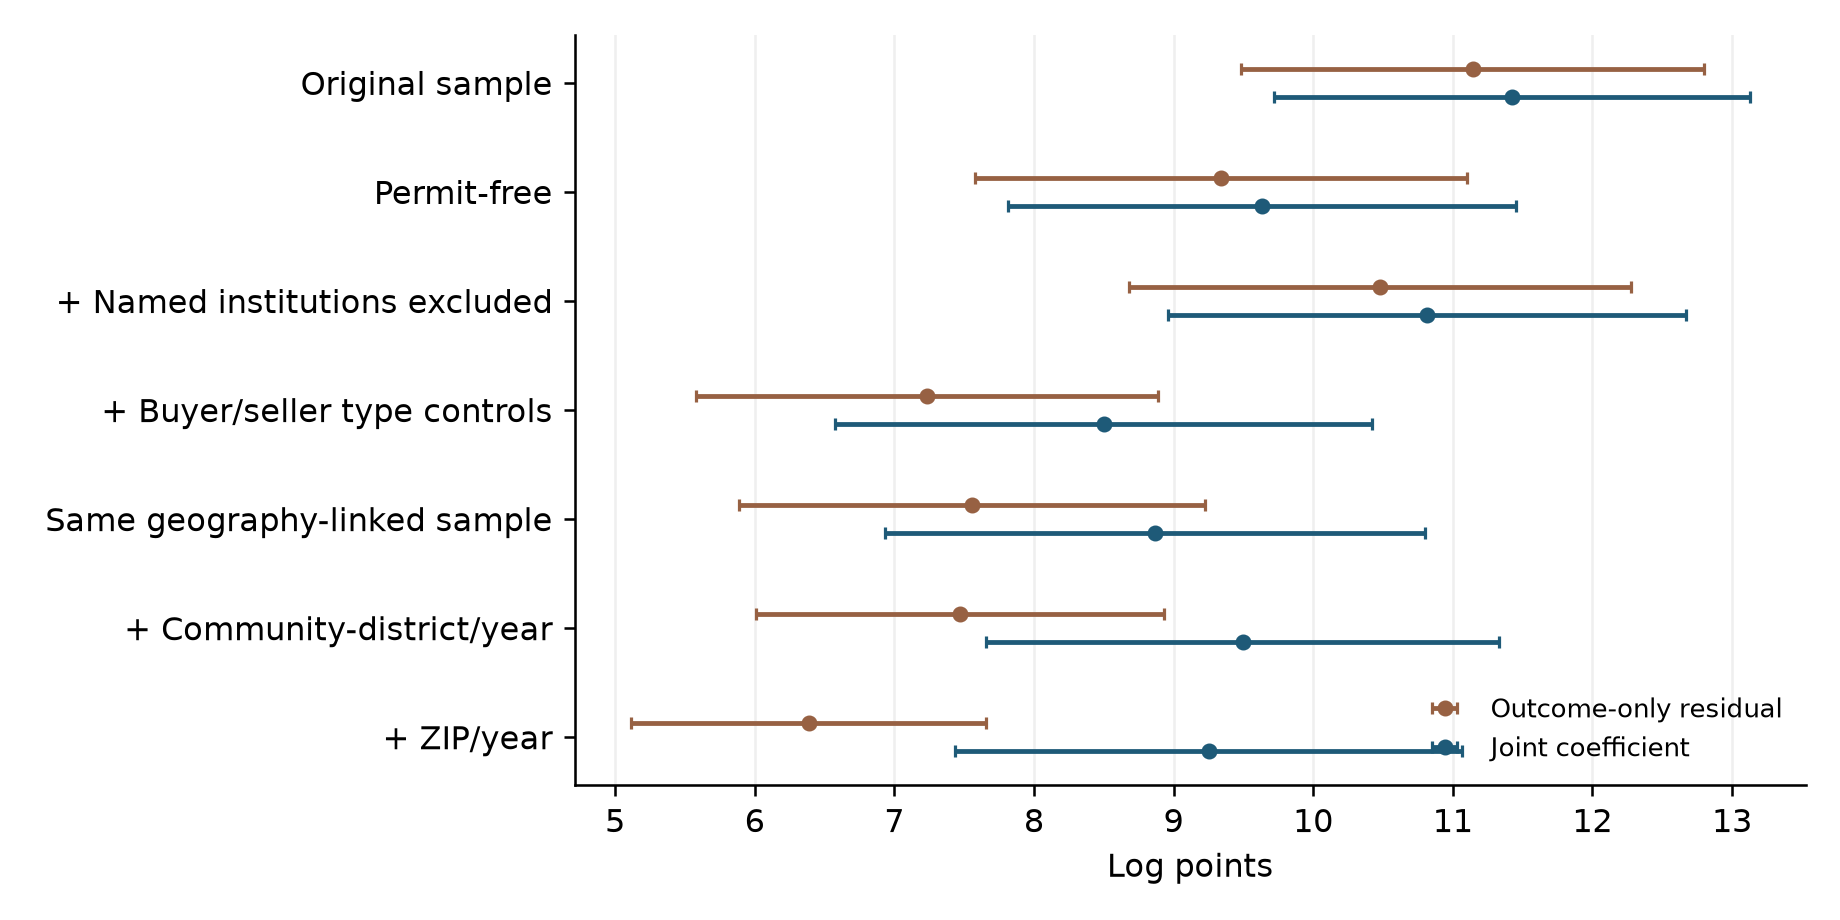
\includegraphics[width=\textwidth]{generated/robustness.png}
\caption{The original residual statistic and joint coefficient across controls}\label{fig:robustness}
\notes{Point estimates and pointwise parcel CR0 intervals. The figure uses one analytic interval method throughout; the principal table also reports common full-refit bootstrap intervals. Community-district/year and ZIP/year are alternative final controls.}
\end{figure}

All specifications' observation influences are summed within the original parcel and stacked before computing covariance. Excluded parcels receive zero influence in that specification. This preserves the covariance induced by overlapping samples. The 999-draw bootstrap resamples original parcel clusters and refits all nuisance controls in four principal specifications using the same draws. It confirms the main joint-coefficient comparison. The high-dimensional residual statistic has a shifted resampling distribution, another reason not to interpret its attenuation as an explained component. Intervals are pointwise and do not incorporate unobserved classification error.

\subsection{Property types and classification sensitivity}
Table~\ref{tab:property} puts houses and condominiums under common borough-quarter controls. The condominium estimate is \CondoGap{} log points, with interval \CondoCI{}. This is a more informative comparison than juxtaposing a heavily restricted house estimate with an unrestricted apartment estimate without identifying their different samples. Even with common controls, differences in ownership form, properties and matching coverage prevent attributing the contrast to standardisation or tax status alone.
\begin{table}[htbp]
\centering\small\singlespacing
\caption{House and condominium contrasts under common controls}\label{tab:property}
\begin{tabular}{lrrrrr}
\toprule
Type & Pairs & $N_{cf}$ & $N_{fc}$ & Joint & 95\% CI \\
\midrule
House & 8,208 & 1669 & 1035 & 11.42 & [9.72, 13.13] \\
Condo & 6,584 & 1228 & 1659 & 0.77 & [-0.01, 1.56] \\
\bottomrule
\end{tabular}
\notes{Both rows use borough-quarter effects and adjacent eligible sales at least 1,095 days apart. All available eligible pairs are used; the cumulative house restrictions are not imposed on the condominium sample. Parcel-clustered CR0 intervals, in log points. Differences in coverage, ownership and financing measurement prevent a causal property-type interpretation.}
\end{table}


The house findings survive narrower and wider financing windows, stable-label restrictions, broader institutional exclusions and consideration-consistent deed matching (Table~\ref{tab:sensitivity}). Window disagreement is an internal consistency measure. Among house sales, strict versus base labels differ for 1,020 observations and wide versus base for 2,193; neither is a known error count. Similarly, passing a consideration match does not establish distress status. A stratified instrument-review queue accompanies the code; no false-positive rate is inferred from these consistency checks.
\begin{table}[htbp]
\centering\small\singlespacing
\caption{Classification and linkage sensitivity}\label{tab:sensitivity}
\begin{tabular}{lrrr}
\toprule
Restriction & Pairs & Joint & 95\% CI \\
\midrule
Financing window: strict & 6,006 & 9.56 & [7.76, 11.36] \\
Financing window: base & 6,006 & 9.25 & [7.44, 11.07] \\
Financing window: wide & 6,006 & 8.60 & [6.77, 10.42] \\
Stable labels at both dates & 5,864 & 9.03 & [7.18, 10.88] \\
Broader institution exclusion & 5,918 & 9.31 & [7.48, 11.13] \\
Unique deed / amount match & 5,798 & 9.23 & [7.44, 11.02] \\
\bottomrule
\end{tabular}
\notes{All rows use the ZIP-year model, with borough-quarter and buyer/seller controls. Log points; parcel CR0 intervals. Stable labels agree between strict and wide windows at both dates. Amount consistency requires a unique nearest deed within 45 days and positive consideration within the larger of one dollar and one percent of the DOF price. These tests concern internal consistency, not classification accuracy.}
\end{table}


\section{Interpreting the financing gap}
\subsection{What the co-operative comparison can establish}
Co-operative share financing is a possible institutional comparison, but the recorded loan measure differs from the house and condominium measure. Timing-unique filing assignments leave 1,765 repeat pairs with an interval including zero; an instrument pilot nevertheless finds a filing that pledges a different unit from its assigned sale. That sale contributes no repeat pair, so rejecting its link leaves the estimate unchanged. A second filing matches the sale unit but lacks independent confirmation of purchase-loan purpose. Appendix~\ref{sec:coopaudit} reports the full assignment and adjacency audit. The co-operative comparison is therefore a measurement sensitivity, not a control group that identifies a mortgage-tax effect.

\subsection{Credit conditions at both sale dates}
If credit conditions shape financing risk, attaching a rate only to the resale misses conditions at the initial transaction. The full house design therefore adds separate terms $F_a(r_a-4)$ and $F_z(r_z-4)$, where $r$ is the latest available weekly Freddie Mac 30-year PMMS rate, in percent, on or before each sale. General time effects absorb common rate levels. The exercise studies financing-specific rate associations.

The baseline slopes have opposite signs across dates (Table~\ref{tab:credit}). Adding separate financing-specific linear calendar trends reduces the first-date association and reverses the second-date sign. Rate movements, time trends and financing composition are difficult to disentangle in these data. The rate evidence consequently does not identify the execution-risk mechanism. The PMMS methodology change on 17 November 2022 is an additional measurement qualification. The augmented model's reference contrasts at 4 percent and the trend origin must not be reported as an unconditional average financing gap.
\begin{table}[htbp]\centering\small
\caption{Credit conditions at both sale dates}\label{tab:credit}
\begin{tabular}{lrrrr}\toprule
Financing $\times$ rate & Without trends & SE & With trends & SE \\
\midrule
First sale & -0.43 & 1.95 & 0.46 & 1.93 \\
Second sale & 2.98 & 0.62 & -1.24 & 1.03 \\
\bottomrule\end{tabular}
\notes{Log points per one percentage point of PMMS rates, centered on 4 percent; 6,006 pairs. Both models include separate uninteracted weekly rates at both endpoints, the full geographic controls and both financing-switch indicators. The second adds separate endpoint financing-specific linear calendar trends. Standard errors cluster by parcel (CR0). Appendix Table~\ref{tab:marketconditions} reports calendar-dependence sensitivity. The headline contrast is estimated in the model without rate interactions.}
\end{table}


\subsection{A conditional seller-model inversion}
Consider a stylised seller comparing a certain cash price $P_c$ with a financed offer $P_f$. Let $q$ be the probability that the financed transaction fails and let $dP_c$ be the loss, relative to the cash alternative, conditional on failure. If continuation following failure is worth $(1-d)P_c$, indifference implies
\begin{equation}
P_c=(1-q)P_f+q(1-d)P_c,
\qquad \frac{P_f-P_c}{P_c}=\frac{qd}{1-q}.
\end{equation}
For an observed log contrast $\pi$, treating that entire contrast as the model premium requires
\begin{equation}\label{eq:inverse}
d^*(q;\pi)=(e^\pi-1)\frac{1-q}{q}.
\end{equation}
This inversion makes the required loss explicit while leaving $q$ as an assumption. Mortgage application denial is not the failure probability of an accepted purchase contract, so national denial rates are not substituted for $q$ here.
\begin{table}[htbp]
\centering\small\singlespacing
\caption{Relisting-loss scenarios implied by the observed contrasts}\label{tab:inversion}
\begin{tabular}{lrr}
\toprule
Failure probability $q$ & Houses: $100d^*$ & Condos: $100d^*$ \\
\midrule
0.1 & 87.2 & 7.0 \\
0.2 & 38.8 & 3.1 \\
0.3 & 22.6 & 1.8 \\
\bottomrule
\end{tabular}
\notes{Scenario calculations from $d^*=(\exp(\pi)-1)(1-q)/q$. Houses use the full geographic joint estimate; condos use the borough-quarter joint estimate. They have different covariate sets and populations. Values of $q$ are illustrative assumptions, not estimated contract-failure probabilities. No common relisting technology is imposed as an empirical fact.}
\end{table}


For common illustrative failure probabilities, the house contrast requires a much greater conditional loss than the condominium contrast. That is a restriction a common-cost explanation must confront, not a proof that the housing market cannot price execution risk. Property-specific liquidity, seller circumstances, the probability of eventually reselling, and differences in the estimated populations can all change continuation values. The mechanism in \citet{hanhong2024} is particularly relevant to that distinction.

Moreover, equation~\eqref{eq:inverse} assumes that the observational contrast is the seller's causal financing premium. The present design does not establish that premise. The table is a sensitivity calculation, not an estimated structural parameter, a lower bound on rents, or a calibration of an optimal cash-purchase charge. A stronger mechanism test would jointly observe financing contingencies, failed contracts, relisting outcomes and prices for comparable properties.

\section{Implications and conclusion}
The central finding is a persistent conditional financing-associated price gap for houses. Its interpretation changes when financing switches and market controls are fitted jointly: local appreciation does not explain away the gap on the common linked sample, while buyer and seller characteristics account for part of it. The smaller condominium contrast under a common specification documents heterogeneity across housing segments, rather than an identified difference in the causal cost of financing.

Three limits matter for this conclusion. Recorded permits cannot capture all changing condition. Institutional-name exclusions remain imperfect measures of foreclosure transfers and subsequent lender resales. Financing-window labels do not independently establish purchase borrowing, and the co-operative pilot demonstrates a concrete collateral-unit mismatch. The reported statistical intervals condition on these measurements. The remaining house contrast cannot be assigned wholly to execution risk, liquidity, taxation or unobserved selection.

For housing policy, the evidence cautions against calibrating a corrective tax from an observed cash--mortgage price difference. Establishing a causal execution component requires information on accepted offers, financing contingencies, failed closings and relisting outcomes, or another credible source of exogenous financing variation. Targeted validation of observations entering the estimating sample would improve the measurement before that interpretation is attempted.

The supplementary transfer-tax analysis examines a separate question about the location of recorded prices. Its strongest period-robust pattern is at the new \$2 million threshold, but no external comparison market has been validated. It does not establish that the mortgage recording tax causes the house gap, nor does it quantify a welfare gain from tax reform. Those questions remain outside the main claim of this paper.

\section*{Declarations}\begingroup\small\singlespacing
Funding, interest and author statements are supplied separately to the editor. AI tools assisted with drafting, literature checking, code development and replication review. The author remains responsible for the analysis and interpretations. Independent human verification of unresolved instrument classifications is not asserted.
\par\endgroup\clearpage\appendix
\section{Joint uncertainty and numerical implementation}
Write $r=M_Xy$ and $m=M_Xc$. The derivative of the residual contrast with respect to an observation weight, evaluated at unit weights, is
\begin{equation}
\operatorname{IF}_{R,i}=m_i r_i-\frac{1\{cf\}_i\bar r_{cf}}{2N_{cf}}+\frac{1\{fc\}_i\bar r_{fc}}{2N_{fc}}.
\end{equation}
The first term accounts for refitting the nuisance projection; the remaining terms account for changes in group denominators. For the joint estimator, let $R=M_XQ$ and $e=M_Xy-R\widehat\beta$. Its coefficient derivative is
\begin{equation}
\operatorname{IF}_{\beta,i}=(R'R)^{-1}R_i'e_i.
\end{equation}
Apply the half-difference contrast, sum within parcel and stack across specifications. The covariance is the cross-product of these stacked cluster influences (CR0). Paired-difference variances use the corresponding covariance terms, rather than treating the two estimates as independent.

A numerical check perturbs five actual parcel weights in the full ZIP-year model, refits the nuisance parameters and verifies both analytic derivatives against finite differences with absolute error below $10^{-7}$. The common bootstrap draws multinomial weights over the 8,127 original house parcels, using seed 20260909, and refits the original, permit-free, linked-party-control and ZIP-year specifications. All 999 draws are retained. Redundant nuisance columns are projected out without interpreting an arbitrary individual fixed-effect solution.

For the notch statistic, an observation contributes $1\{above\}/N_{above}-1\{below\}/N_{below}$ to a log-ratio derivative. Differencing periods and placebo prices before summing cluster scores incorporates overlapping windows. No multiple-testing correction is applied; all intervals are pointwise. These covariance calculations condition on the observed linkage and classifications.

\section{Replication map and classification definitions}
The master script \texttt{code/reproduce.py} parses the preserved rate extracts, rebuilds enriched pairs, estimates the house models and bootstrap, audits co-operative assignments, recomputes the notch and financing samples, performs numerical checks and regenerates manuscript exhibits. The replication README contains exact setup instructions, package versions and a file-level exhibit map. Archived original inputs remain distinguishable from newly retrieved extracts and derived outputs.

Table~\ref{tab:cumulative}, Table~\ref{tab:paired} and Figure~\ref{fig:robustness} derive from the repeat-sale results and joint bootstrap outputs. Table~\ref{tab:property} recomputes both property types from the archived panel. The co-operative, credit, classification, notch and charm tables map to their named analysis scripts. Table~\ref{tab:inversion} is computed directly from the displayed formula and identified point estimates. Figure~\ref{fig:annual} uses annual output from the same local count-ratio code.

The loan windows in the house/condominium input are document-based purchase-window proxies; the co-operative windows concern personal-property recording dates. These do not have identical coverage or timing interpretation. The party classifications are reproducible regular-expression categories, not verified persons, beneficial owners or distressed sales. Unknown party records remain explicit rather than being silently classified as individuals. The release retains audit fields and review queues so subsequent adjudication can be versioned without overwriting the underlying rules.


\section{Co-operative assignment and adjacency audit}\label{sec:coopaudit}
\subsection{Why the co-operative comparison requires an audit}
A building-level UCC filing is not inherently a particular unit buyer's purchase loan. Multiple sales and filings can occur near each other, some sales lack recovered unit identifiers, and filings can concern other credit events. The fresh co-operative extract therefore includes all observed prices and incomplete-unit records when counting possible competitors for a filing, rather than using only the estimation sample.

The audit reconstructs the expanded count rule: for a sale at date $d$, count eligible sales within $d\pm45$ days and filings within $[d-60,d+135]$. A zero filing count is coded cash; a filing count at least as large as the sale count is coded financed; the remainder is ambiguous. The expansion is consequential. Of 60,496 purchases labelled financed, 4,385 have no filing in the base $[-15,+90]$-day window. Counting all observed competing sales also changes assignments.

The alternative rules require exactly one candidate filing and exactly one observed sale eligible to claim that filing. The narrow, base and wide windows are $[-15,+30]$, $[-15,+90]$ and $[-15,+180]$ days. Documents linked to multiple parcels are excluded. These conditions prevent reuse of a supposedly unique filing, but cannot identify its debtor, collateral unit or purchase purpose. Zero candidates still means no matched record, not proven cash.

Adjacency is determined using all observed known-unit sales before dropping endpoints with ambiguous financing or out-of-band prices. The audit finds 271 pair keys from the reconstructed older procedure that bridge an intervening observed unit sale. Table~\ref{tab:coop} uses the corrected ordering in every row. Base timing uniqueness leaves 1,765 pairs in 1,082 buildings. Its interval includes zero, as do the narrow and wide alternatives. This is compatible with a small co-operative contrast within selected, differently measured samples; it is not evidence that the mortgage recording tax causes the house gap.
An instrument pilot makes the remaining linkage problem concrete. Among two timing-unique candidates inspected, one filing names the recorded sale unit; the other pledges a different unit in the same building. The latter sale contributes no repeat pair, so rejecting its filing link does not change Table~\ref{tab:coop}. The matching case still lacks independent confirmation of purchase-loan purpose. These observations demonstrate a failure mode, not a population error rate, and preclude treating timing uniqueness as validated financing.
\begin{table}[htbp]
\centering\small\singlespacing
\caption{Co-operative assignment sensitivity}\label{tab:coop}
\begin{tabular}{lrrrrr}
\toprule
Assignment rule & Pairs & $N_{cf}$ & $N_{fc}$ & Joint & 95\% CI \\
\midrule
Expanded count rule & 5,839 & 247 & 602 & -1.18 & [-3.11, 0.75] \\
All competing sales & 5,261 & 229 & 576 & -0.89 & [-2.77, 1.00] \\
Unique timing: narrow & 2,840 & 441 & 537 & -0.41 & [-2.00, 1.18] \\
Unique timing: base & 1,765 & 219 & 252 & -1.42 & [-3.70, 0.86] \\
Unique timing: wide & 1,265 & 108 & 143 & 0.09 & [-2.99, 3.17] \\
\bottomrule
\end{tabular}
\notes{Log points and building-clustered CR0 intervals. Every row forms adjacency using all observed known-unit sales before dropping ineligible endpoints and ambiguous financing. Timing uniqueness does not establish debtor identity or purchase purpose. No matched filing is a cash proxy, not proof of an unlevered purchase. Estimates use the September 2026 co-operative extract.}
\end{table}



\section{Supplementary transfer-tax evidence}\label{sec:transferappendix}
\subsection{Transfer-tax thresholds and statutory liability}
The city's residential Real Property Transfer Tax (\citealp{nycrptt}) rises from 1 percent to 1.425 percent \emph{above} \$500,000. A price of exactly \$500,000 is therefore on the lower-tax side. New York's mansion tax under \S1402-a is 1 percent when consideration is \$1 million or more and applies to the whole taxable consideration. Both taxes create jumps in total liability rather than continuous marginal brackets.

The 2019 changes created additional discontinuities (\citealp{nyreform2019}). Section 1402-b adds 0.25 percent for residential conveyances at \$2 million, rising to 0.50 percent at \$3 million. At \$3 million, the state base transfer rate under \S1402 also rises from 0.40 to 0.65 percent. The combined new jump there is thus half a percentage point. The reform applies to conveyances on or after 1 July 2019, with the statutory exception for qualifying binding contracts entered into on or before 1 April. The main pooled comparison omits 2019; supplementary comparisons use its second half and fourth quarter, with grandfathering unresolved.\footnote{See New York Tax Law \S\S1402, 1402-a, 1402-b and the New York State Department of Taxation and Finance's 2019 transfer-tax guidance. Higher thresholds exist but are outside the main comparison.}

The supplemental tax under \S1402-b is primarily payable by the \emph{grantee}. If the grantee fails to pay or is exempt, the grantor has a duty to pay; failure to pay can give rise to joint and several liability. The base transfer tax is primarily a grantor obligation. These provisions identify legal payment duties. They do not reveal how negotiation reallocates the burden between buyers and sellers. A discontinuity shared across taxes with different primary payers cannot identify separate incidence from the price distribution alone.


\subsection{A local price-distribution comparison}
This supplementary exercise follows \citet{kopczuk2015} and \citet{best2018} in examining price responses near transfer-tax thresholds. Its incremental evidence concerns the 2019 NYC reform, not a new general demonstration that housing taxes can affect reported prices. The shape of a tax schedule is a separate question from what causes the financing-associated price gap. A jump in total liability makes nearby reported prices carry sharply different taxes. The 2019 reform provides a dated change at \$2 million and \$3 million, while the pre-existing \$500,000 and \$1 million thresholds provide descriptive comparisons.

For threshold $X$, define the count ratio $R_{Xt}$ using an above window $[X,X+100{,}000)$ and a below window $[X-150{,}000,X-50{,}000)$. At \$500,000 the above window excludes $X$ because that exact price remains on the lower-tax side. The gap immediately below the threshold keeps the principal denominator away from the most obvious bunching region, but does not prove it is unaffected by behavioural responses.

Let pre denote 2016--2018 and post denote 2020--2025. The statistic is
\begin{equation}
\widehat\Delta_X=\bigl(\log R_{X,post}-\log R_{X,pre}\bigr)
-\frac14\sum_{p\in\mathcal P}\bigl(\log R_{p,post}-\log R_{p,pre}\bigr),
\end{equation}
with $\mathcal P=\{1.5,1.75,2.25,2.5\}$ million dollars. These are placebo \emph{prices}, not untreated markets. A causal reform interpretation requires absent-reform local distribution changes at the threshold to track those at the comparison prices, and requires spillovers not to differentially contaminate the windows. The always-treated thresholds cannot simply be presumed valid controls either.

The 2019 exclusion avoids combining announcement, implementation and grandfathered contracts within a single treatment period. It does not remove pandemic-era changes or long-run shifts in the luxury market. The price windows and placebo choices are reported alongside annual patterns and sample sensitivity so those concerns remain assessable.

Supplementary comparisons separate 2020--2021 from 2022--2025 and examine 2019 H2 and Q4 against the same months of 2016--2018. The latter comparisons provide pre-pandemic evidence but cannot separate grandfathered contracts. All five post-period choices, three bandwidths and three thresholds are reported, rather than selecting a preferred result after inspection.

\subsection{Results and what the counts mean}
Table~\ref{tab:notches} reports negative relative changes at the new \$2 million and \$3 million thresholds. The \$1 million comparison is close to zero and the \$500,000 comparison is positive. Confidence intervals account jointly for overlapping price-window contributions and repeated parcels. Where parcel identifiers are missing, observations are grouped conservatively within borough; results restricted to known parcels are supplied in the replication outputs.
\begin{table}[htbp]
\centering\small\singlespacing
\caption{Changes in local price-count ratios around transfer-tax thresholds}\label{tab:notches}
\begin{tabular}{lrrr}
\toprule
Threshold & Log-ratio change & 95\% CI & Relative change (\%) \\
\midrule
\$0.5m & 0.194 & [0.13, 0.26] & 21.4 \\
\$1m & 0.017 & [-0.07, 0.11] & 1.7 \\
\$2m & -0.339 & [-0.47, -0.21] & -28.7 \\
\$3m & -0.623 & [-0.86, -0.39] & -46.4 \\
\bottomrule
\end{tabular}
\notes{The 2016--2018 to 2020--2025 change in the log above/below count ratio, less the mean change at four placebo prices (\$1.5m, \$1.75m, \$2.25m, \$2.5m). The above window is $[X,X+100{,}000)$ and the below window $[X-150{,}000,X-50{,}000)$; at \$500,000 the above window excludes $X$, where the lower city rate still applies. All 2019 observations are omitted. Joint parcel CR0 intervals include overlapping-window covariance. Relative change is $100(\exp(\widehat\Delta)-1)$, not lost sales or welfare.}
\end{table}


The negative new-threshold contrasts survive using each placebo separately and excluding missing parcel identifiers. Collapsing identical parcel/date/price tuples is an additional sensitivity, not verified deduplication: the archived price sample lacks units and such tuples can represent different co-operative sales. Matched house/condominium comparisons retain negative pooled new-threshold estimates, while the condominium-specific \$2 million interval includes zero. It would be incorrect to claim equally precise evidence across property types.

\begin{figure}[htbp]\centering
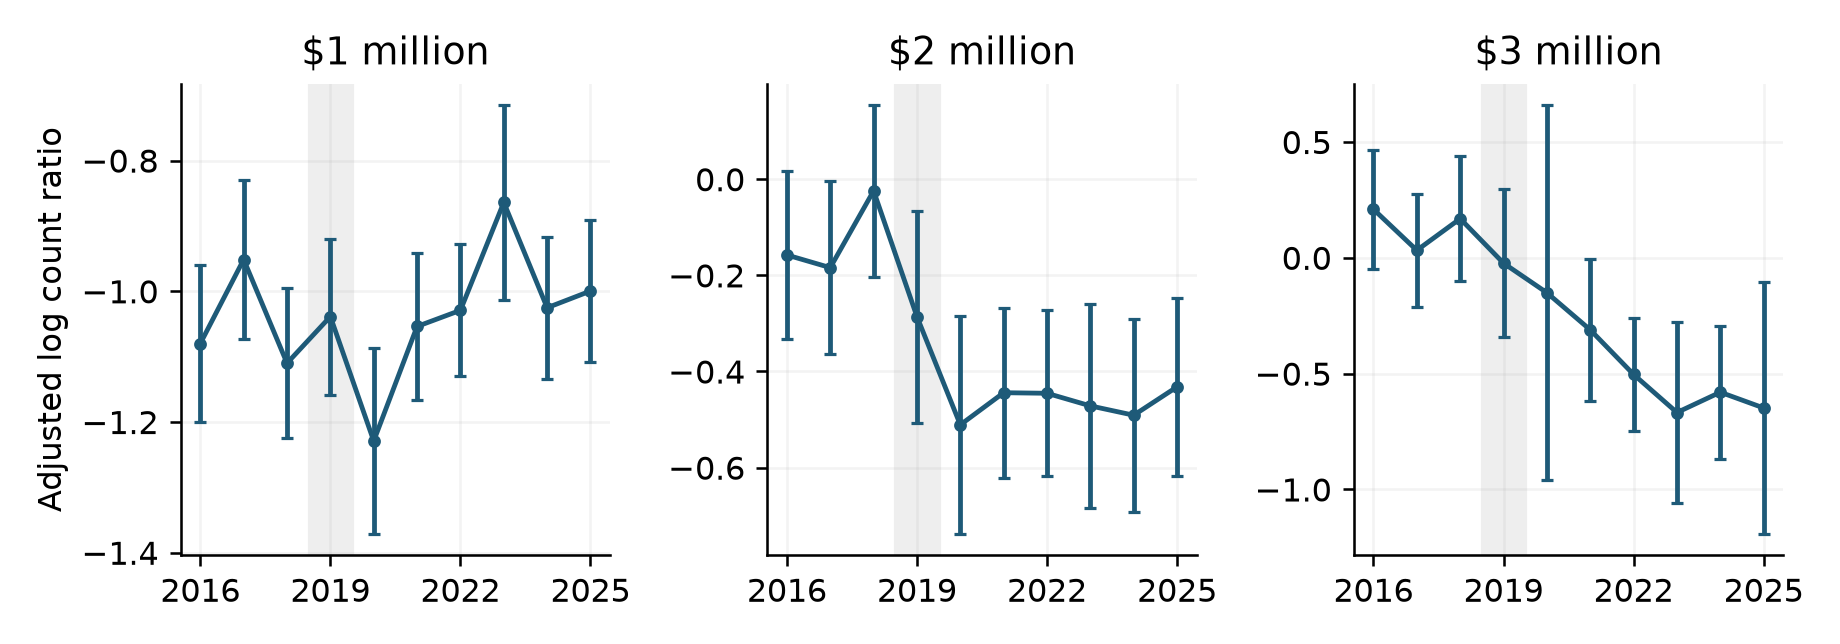
\includegraphics[width=\textwidth]{generated/annual.png}
\caption{Annual local count ratios relative to placebo prices}\label{fig:annual}
\notes{Levels of the annual log count ratio less the mean at the four placebo prices, with pointwise parcel CR0 intervals. The shaded year, 2019, is omitted from the pooled pre/post statistic. Levels are not event-study coefficients normalised to a pre-reform reference year.}
\end{figure}

The additional period checks are most consistent at \$2 million (Appendix Table~\ref{tab:targetedperiods}). At the main bandwidth, the contrast is $-0.337$ in 2022--2025 and $-0.380$ in the season-matched 2019 H2 comparison; both pointwise intervals exclude zero. At \$3 million, the 2019 H2 and 2020--2021 intervals include zero, while Q4 is negative with only 18 post-period transactions in the above window. Both new-threshold contrasts remain negative across the three bandwidths in the pooled comparison, with appreciably different magnitudes. Pre-period stability tests do not reject at either new threshold, but three pre-years offer limited power and the narrow \$1 million comparison rejects stability. These diagnostics strengthen the case for a dated local price-distribution change at \$2 million without establishing a causal elasticity.

The reported percentage transformation is a proportional change in a relative count ratio. It is not the percentage of all transactions destroyed. Buyers and sellers may reprice, change timing, choose other properties, or stop transacting. Those responses need different counterfactual quantities to be separated. For that reason, the paper does not convert the local count changes into deadweight loss or infer an aggregate revenue effect.

\subsection{Charm prices, legal payers and economic incidence}
Prices one dollar below a threshold provide a complementary description of price location. To keep financing comparisons coherent, Table~\ref{tab:charm} uses exactly the same 2020--2025 four-borough house/condominium universe at each threshold. A linear probability regression compares financing at $X-1$ and $X$, conditioning on threshold, borough-year and property-type-year effects.
\begin{table}[htbp]
\centering\small\singlespacing
\caption{Financing composition at exact and one-dollar-below prices}\label{tab:charm}
\begin{tabular}{lrrrr}
\toprule
Threshold & Selected sales & $X-1$ sales & Difference & 95\% CI \\
\midrule
\$0.5m & 859 & 40 & 3.10 & [-11.24, 17.45] \\
\$1m & 441 & 377 & 11.59 & [-0.74, 23.92] \\
\$2m & 295 & 90 & 14.14 & [2.80, 25.48] \\
\$3m & 129 & 47 & 36.03 & [20.09, 51.97] \\
\bottomrule
\end{tabular}
\notes{Common 2020--2025 four-borough house/condo sample. Difference in financed share (percentage points), $X-1$ minus $X$, from a linear probability model with threshold, borough-year and property-type-year effects. Parcel CR0 intervals. Exact-price cells are small and selected. At \$500,000 both prices face the lower city rate. These are financing-composition contrasts, not estimates of economic incidence.}
\end{table}


Financing shares are higher at the one-dollar-below prices at the new thresholds, but the selected cells are small. These contrasts can reflect liquidity, negotiations, buyer composition or recording conventions. They cannot establish which party economically bears a tax. At \$2 million the new supplemental liability is primarily the grantee's; at \$3 million both grantee and grantor statutory components change. Their joint appearance in recorded prices does not isolate either component's causal effect. At \$500,000, both $X-1$ and $X$ are on the lower-tax side, which makes an identical tax-avoidance interpretation especially inappropriate.

\subsection{Tax-design considerations beyond the financing-gap estimates}
The evidence motivates evaluating two design objectives separately. Financing neutrality concerns whether otherwise similar acquisitions face different statutory charges because one records a real-property mortgage. Schedule continuity concerns whether an arbitrarily small price change produces a discrete jump in total tax. Neither objective determines an optimal revenue level, distributional target or corrective rate.

Reducing mortgage recording taxes would narrow the statutory financing difference, but would also require an explicit fiscal counterpart. Some recording-tax receipts are dedicated to transportation under Tax Law \S261, including receipts associated with \S253(2). A reform must specify how replacement revenue reaches the relevant beneficiaries, rather than infer a precise MTA loss from a headline tax rate applied to this sample. The paper's transaction counts and observed mortgage labels do not reconstruct the full revenue base or instrument-specific exemptions.

One possible replacement is a transaction schedule with continuous total liability,
\begin{equation}
T(P)=\int_0^P \tau(s)\,ds,
\end{equation}
where a bounded marginal rate $\tau(s)$ can increase at specified thresholds without making $T(P)$ jump. The precise mathematical advantage is local: as prices approach a threshold from either side, the tax difference tends to zero. The schedule removes the discrete tax reward for relocating a recorded price just across that threshold. It does not eliminate all transaction discouragement, avoidance, reporting responses or responses to marginal-rate kinks.

A financing-neutral replacement would also need a clear scope for co-operative shares, ownership changes, exemptions and treatment of existing debt. Any chosen rates should be evaluated against an explicit revenue and distributional counterfactual. The present results supply reasons to investigate that design; they do not justify a particular surcharge on cash buyers, recover its welfare gain, or establish that equalising statutory charges necessarily improves welfare in a market with other frictions.


\section{Targeted instrument pilot and reform checks}\label{sec:pilot}
The consolidated supplement reuses the preserved analysis inputs. Four queued cases were inspected through the public ACRIS image viewer on 10 September 2026: one broad-only house flag, one specific-institution house flag, and two timing-unique co-operative assignments. Saved page images, document identifiers, review notes and source hashes accompany the supplement. These are AI-assisted document readings awaiting independent review. The 90-house and 90-co-operative queues remain incomplete; their sampling weights must not be applied to this selectively continued four-case pilot to estimate error rates.

House deed 2023051600851001 recites the lender's acquisition under referee deed 2019020500740001. The earlier operative instrument describes a mortgage foreclosure and conveyance to the lender; the later transaction is consistent with a lender resale. The broader name rule flags the sale whereas the narrower rule does not. House deed 2019093000695001 is explicitly a referee's deed in foreclosure and is already caught by the narrower institutional-buyer rule. Both source cover records use DEED metadata. These findings distinguish mechanisms within institutional flags without measuring property condition or the effect of distress on prices.

For co-operative filing 2025020500312001, the sale unit and collateral designation both identify 7AB, but purchase-loan purpose remains unverified. Filing 2020020400882001 pledges unit 4E, whereas its timing-assigned sale identifies 1CD. The preserved sale extract contains only one observation for that latter unit; the false link therefore affects no repeat pair. It is rejected as evidence for that sale's financing, without relabelling the sale as cash. A timing-only rule cannot resolve this unit mismatch even when it has no observed competing sale.

\begin{table}[htbp]\centering\small
\caption{Reform comparisons by post period}\label{tab:targetedperiods}
\begin{tabular}{lrrrr}\toprule
Post period & $\Delta_{2m}$ & 95\% interval & $\Delta_{3m}$ & 95\% interval \\ \midrule
2020--2025 & -0.339 & [-0.469, -0.209] & -0.623 & [-0.858, -0.388] \\
2020--2021 & -0.344 & [-0.518, -0.170] & -0.387 & [-0.781, 0.006] \\
2022--2025 & -0.337 & [-0.478, -0.195] & -0.729 & [-0.975, -0.482] \\
2019 H2 & -0.380 & [-0.723, -0.037] & -0.304 & [-0.760, 0.151] \\
2019 Q4 & -0.628 & [-1.062, -0.193] & -0.752 & [-1.393, -0.111] \\
\bottomrule\end{tabular}
\notes{Changes in log above/below price-count ratios less the mean change at four placebo prices; $100{,}000$ windows. Reference period: 2016--2018, restricted to the same calendar months for the 2019 rows. Intervals use joint parcel-cluster CR0 scores and are pointwise. The 2019 rows may include grandfathered contracts. Periods overlap; separate significance levels do not test differences between periods. All 45 period/bandwidth comparisons are retained in the supplement.}
\end{table}

The supplement reports all 45 period/bandwidth comparisons, nine joint pre-period stability tests and six geographical diagnostics. The pooled new-threshold contrasts remain negative separately in Manhattan and the other boroughs at the main bandwidth. This addresses one coarse composition concern, not all within-market shifts. Confidence intervals combine period and placebo contributions before parcel clustering; overlapping windows are therefore accounted for. No multiplicity correction is applied. The additional scripts, preserved instrument evidence and outputs are included in the consolidated replication package. Its README distinguishes the inherited clean analysis run from the submission build.

\begingroup\small\singlespacing\raggedright\bibliography{references_anonymous}\endgroup
\end{document}
